\documentclass[10pt]{article}\usepackage{graphicx,psfrag}\usepackage{amsmath}
\begin{document}\thispagestyle{empty}\begin{figure}
\psfrag{function evaluations}[][]{\small \# function evaluations}
\psfrag{mean fitness}[][]{\small mean fitness}
\psfrag{CMAES}[][]{\small ~~~~~~~~~~~ $(\mu_I,\lambda)$CMA-ES}
\psfrag{Poly-2}[][]{\small ~~~~~~~~~ Poly, $\overline{\ell}=\lambda$}
\psfrag{Poly-2-ell}[][]{\small ~~~~~~~ Poly, $\overline{\ell}=2\lambda$}
\psfrag{n=2}[][]{\small $n=2$}
\psfrag{n=5}[][]{\small $n=5$}
\psfrag{n=10}[][]{\small $n=10$}
\psfrag{n=20}[][]{\small $n=20$}
\noindent{\Large
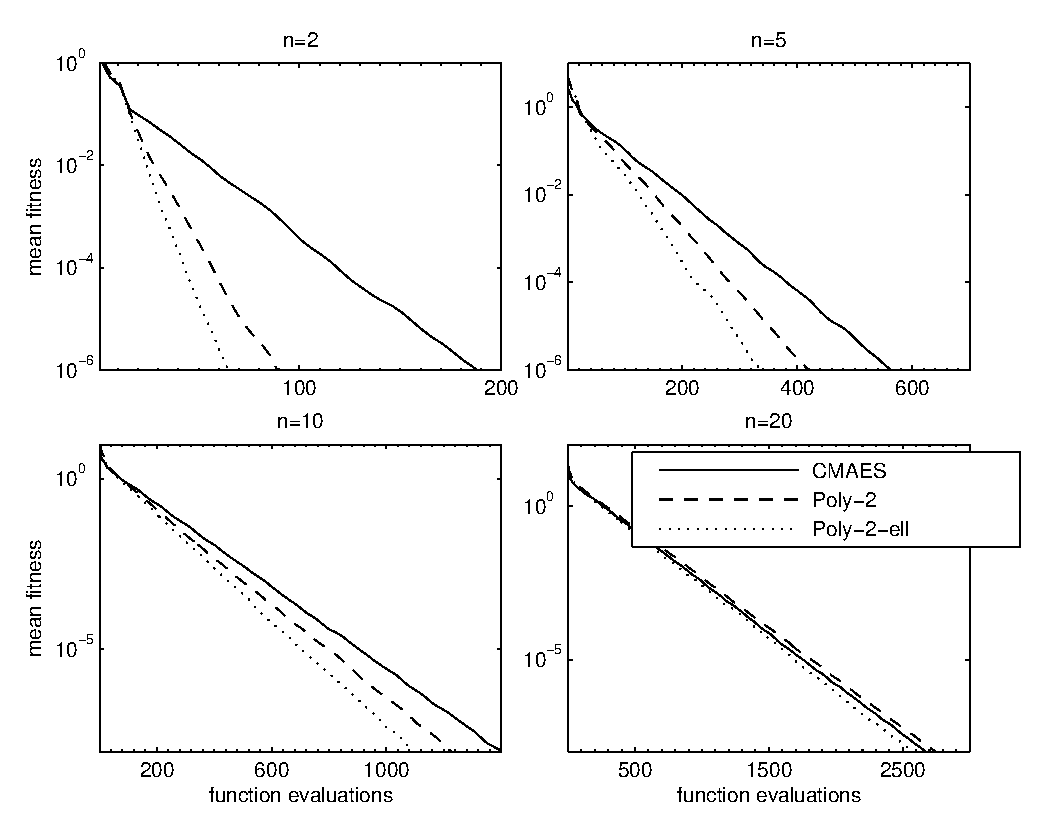
\includegraphics[width=12cm]{sphere2.eps}}
\end{figure}\end{document}
